\hyperref[sec:sec29]{\section{為什麼香港會有這麼多民意調查?}}
\label{sec:sec27}

其實香港的民意調查已經不算多,在美國就可以每週有多個民調機構發布總統支持度的民調,香港的行政長官民調就沒有那麼頻密。不過,相對於其他地方,由於香港政制本身的缺陷,使得民調在香港扮演了不一樣的角色,甚至自己成為了政治爭議的主角。

即使在一個正常的民主社會,民調本身也有很重要的地位。如果政府民望持續低迷,可以警剔執政者盡快改善,不用等到選舉時被趕下台才後悔。在野黨也可以按民意的走向準確出擊,更有效地向公眾揭露政府的失誤。民意調查可以讓一般人的聲音繞過菁英階層呈現,畢竟在未有民意調查的年代官員或意見領袖可以輕易地自稱代表「沉默的大多數」,但在民調數據面前就不能這樣亂說。而從公共政策分析的角度來看,民調更可進一步解拆社會中不同階層類別(如年齡、性別和種族)對同一件事情的不同意見,無論對學術研究或政策制訂也十分重要。

落在香港,民調的角色卻有所爭議。由於選舉制度的問題,行政長官不是普選產生,固然不能自稱得到民意的授權。即使是立法會,也因為有功能界別的存在以至決議經常違反民意。如是者,一種意見認為民調在香港的作用不如正常民主社會,因為它不能直接影響政治過程,未能對執政者構成壓力,民望低迷的董建華也可在二零零二年在毫無對手下連任就是一例。

不過,正正因為選舉制度的缺陷,即使政府能在立法會「數夠票」通過,也不可以自以為得到民意的支持。直選產生的立法會議員也可以聲稱他們才代表民意,以此和政府抗衡。由於沒有公平選舉作為民意認授的客觀訟裁者,民調就往往被理解成為決定「誰才真正代表民意」的間接方式。有意見甚至認為由於香港政府不像一個正常的民選政府一樣得到民意認授,不能以曾經得到選票授權而強推短期內不受歡迎的政策,所以抵擋短期民意波動的能力反而較低,也使得政府反而不敢推行一些較具爭議的重要改革。

自特區成立以來,香港各個民調機構都有追蹤調查各種重要的社會指標,例如香港人的身分認同,對世界各地人民和政府的觀感,以及對一國兩制的信心等等。最為傳媒注意的,則是對行政長官的民望調查。如前文所述,各任行政長官的評分都離不開從上任起即日走下坡的趨勢(見\hyperref[sec:sec19]{問題十九}),使得民調報告有時會成為異議者攻擊政府的武器,也因而引來支持政府者的批評,例如質疑民調的可信性。符合社會科學嚴格標準的民調,如果因為結果不符合個別的政治立場而受到批評,本身是件十分可悲的事件。畢竟,民調在社會的功能就有如一個溫度計,只為準確反映天氣冷熱。如果對天氣不滿,而去責怪或抹黑溫度計本身,只不過是掩耳盗鈴,長遠對執政者沒有好處。

就民調和執政者之間的關係,特區成立以來最嚴峻的一役可謂「路祥安事件」。港大民意研究計劃總監鍾庭耀在二零零零年七月於報章撰文指控行政長官透過某些渠道施壓要求他停止對行政長官和特區政府表現的民調,引發公眾嘩然。鍾庭耀及後透露港大校長鄭耀宗曾透過副校長黃紹倫兩次向他傳話,表明董建華對他進行的民調不高興,還稱可能會「陰乾」其研究經費。及後鄭耀宗承認行政長官的高級特別助理路祥安曾經約見他討論相關民調。就此,港大校委會通過進行公開調查聆訊,結論直指鄭耀宗干預學術自由。在校內和社會輿論的龐大壓力下,鄭耀宗和黃紹倫均於校委會討論是否接納報告前辭職。自此之後,民調的中立地位便成為輿論的關注對象。

反過來,近年來又有民調機構被輿論批評為不中立和不公正。例如香港民意調查中心由於附屬被認為是親建制的一國兩制研究中心,其公佈對政府有利的民調結果時就會受到質疑,認為只是製造民意方便向中國大陸輸出假象。另一組織香港研究協會則常被質疑實為替建制派政黨服務,而其選舉日所作的票站調查有否被非法挪用為政黨配票的工具,更是每次選舉的常見話題。儘管這些指控往往難以證實,但傳言不斷已足以影響民調的正常運作。例如有輿論會鼓吹每當遇到民意調查,便應胡亂作答或刻意回答建制陣營想聽到的答案,以圖擾亂調查結果。但當大學的專業民調也受到這些做法干擾,無法進行客觀調查時,受損的其實是整個社會。

\begin{figure}[htbp]
    \centering
    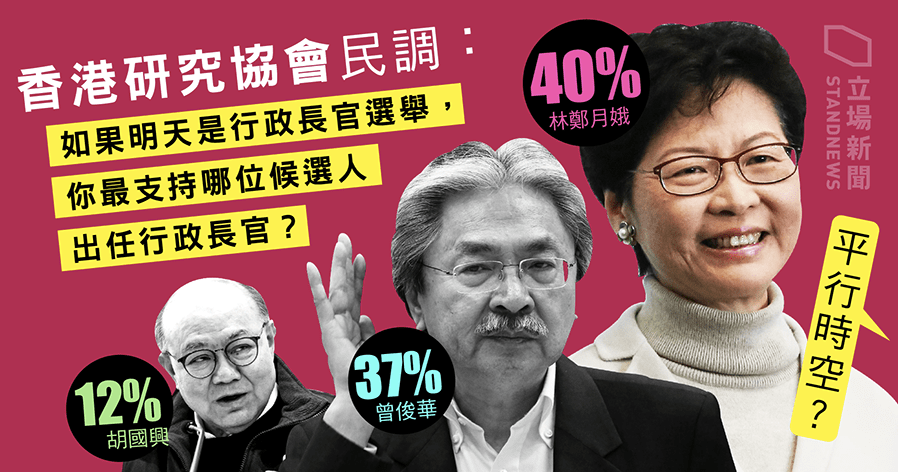
\includegraphics[width=0.7\textwidth]{c27/h-klesson1-044.png}
    \caption{有民調機構被認為發放了不準確的結果,影響輿情} 
\end{figure}

值得注意的,是除了民間做的民調之外,政府自己也會做各式各樣的民調和社會研究,以免與公眾情緒和訴求脫節。不過在缺乏政黨輪替壓力的前提下,政府和親政府輿論有多重視這些民調和社會研究就很難保證。過去就不乏政府和親政府輿論推銷一套觀點,但所做的調查卻否定了這些觀點。例如就中學通識科對學生政治態度的影響,就有建制陣營的議員提出學科使得學生更為靠近本土觀點,應該整頓;但由中央政策組資助的學術調查卻顯示,喜愛通識科的學生不更為靠近本土觀點,而且更認同接納新移民,可見學科鼓勵的明辨思考能使學生更為包容。又曾有建制陣營政黨邀請大學做民調,研究青少年的國民身分,結果發現青少年對中國大陸的批評並非出於無知。會出現這些和資助者相反的結論,是因為大學的研究單位和資助方簽訂合約的時候,通常規定對方不能選擇性發表結論,而要全套結果如實發表。

儘管大學的研究單位一般都十分努力通過學術專業來保持其公信力,但仍然常常會受到質疑。其中一個原因,是正正基於他們的中立地位,所以願意接受非建制陣營的委託,成為一些非建制陣營活動的中立仲裁者,例如主持立法會選舉的非建制陣營初選。但站在建制陣營輿論的立場,卻會認為這就是這些大學研究單位並不可信的「證據」。

面對此得壓力,香港的大學能否繼續支持民調,漸成疑問。民調的一個特性,是往往要長時期的連續監察,例如同一條問題每半年問一次,連續問二十年,才能在研究上發揮效用。要持續地支持民調運作,由大學視為社會基礎研究來支持是比較可行的安排。最近值得注意的發展,就是港大民研隨著總監鍾庭耀退休之後,能否維持其特色和獨特性的問題。現時的安排,是把港大民研從大學獨立出來,成立「香港民意研究所」,以眾籌方式生存。

民調是理解社會的重要工具。但要善用民調,應同時理解其功能和限制。概念上,民調所述的僅為公眾在有限選項間的綜合態度,不代表公眾本身理解這些議題和選項,而這些選項本身也可能有所不足,問題設定本身和對人口參數的各種假設可以大幅影響結果。民調本身十分昂貴,一般民間組織難以負擔,即使對官方所述的民意有所質疑也未必能另做民調核實。近年來越來越多少人設有家居電話,平時只用手提電話通信,使得民調機構也要學習調整調查方法來保持代表性。近年更興起網上輿情監察,但其研究方法和代表性尚未見成熟。

最後,有數據不一定有真相。就算數據搜集的過程能做到客觀公正,片面的解讀卻會製造更多問題。例如近年社會輿論走向兩極化,對一些重大議題的態度往往是極不同意和極同意的較多,如果有不誠實的分析只看總平均數,削去兩極化的特性,便會忽視了民意其實不止得一個。民調是一個很有用的社會分析工具,但如何用這個工具和達到什麼目的,則是一個政治問題,而這點又離不開香港本身政治制度的缺陷了。

\rule[-10pt]{15cm}{0.05em}

伸延閱讀:

趙永佳、沈國祥、葉天生(2017):〈特區政府的民望調查〉,載於張妙青、趙永佳編《香港特區二十年》,香港:香港中文大學香港亞太研究所。

Currie J, Petersen CJ, Mo KH (2006) The Robert Chung Affair, \textit{Academic Freedom in Hong Kong}. Oxford: Lexington Books.

網上資源:

\href{https://thestandnews.com/politics/平行時空-香港研究協會民調-林鄭領先曾俊華/}{立場報道(2017)香港研究協會民調:林鄭領先曾俊華,2017年3月13日}